\documentclass{article}
\usepackage{graphicx}
\usepackage{booktabs}
\usepackage{subcaption}
\usepackage{tikz}
\usetikzlibrary{spy}


% Examples of custom/rare figures with mixed content

\begin{document}

% see issue ar5iv#83
\begin{table*}[t]
  \footnotesize
  \resizebox{0.36\columnwidth}{!}{
  \begin{minipage}[t]{0.4\textwidth}
    \begin{tabular}{cc}
      \toprule
      Head & Meta \\
      \midrule
      Body & Content \\
      \bottomrule
    \end{tabular}
  \end{minipage}}
  \hspace{15em}
  \resizebox{0.36\columnwidth}{!}{
  \begin{minipage}[t]{0.4\textwidth}
    \begin{tabular}{cc}
    \toprule
    Head 2 & Meta 2 \\
    \midrule
    Body 2 & Content 2 \\
    \bottomrule
    \end{tabular}
  \end{minipage}}
  \caption{table with two resized, minipage, tabulars}
\end{table*}
\clearpage

% \includegraphics as a node in tikz, see ar5iv#215

\begin{figure*}
  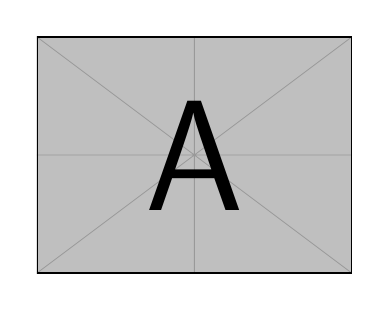
\begin{tikzpicture}
    \begin{scope}[spy using outlines={rectangle,blue,magnification=2.5,size=3cm}]
    \node {	\includegraphics[height=3cm]{example-image-a}};
    \end{scope}
  \end{tikzpicture}

  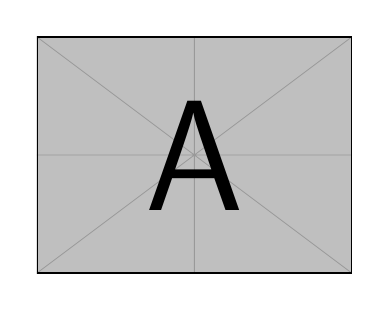
\begin{tikzpicture}
    \begin{scope}[spy using outlines={rectangle,blue,magnification=2.5,size=3cm}]
    \node {	\includegraphics[height=3cm]{example-image-a}};
    \end{scope}
  \end{tikzpicture}
  \caption{tikz nodes with includegraphics}
\end{figure*}
\clearpage

% math array with subfloat
\begin{figure}
  $ \begin{array}{cc}
    \subfloat[]{\includegraphics[width=3cm]{example-image-a} \label{array:subfig1}} &
    \subfloat[]{\includegraphics[width=3cm]{example-image-a} \label{array:subfig2}}
  \end{array} $
  \caption{math array figure}
  \label{array:fig}
\end{figure}
Testing \ref{array:subfig1} and \ref{array:subfig2} inside \ref{array:fig}.
\clearpage

% listing, itemize, enumerate, inline math, display math, para text
% footnotes,


\end{document}